% Copyright (c) 2015-2017, AIT Austrian Institute of Technology GmbH.
% REM All rights reserved. See file POWERFACTORY_FMU_LICENSE.txt for details.

\chapter{Examples}
\label{sec:examples}

This chapter gives examples of exporting FMUs from \pf models as described in Section~\ref{sec:export}.
All the examples use the same simple network model (Figure~\ref{fig:test_model}) and produce the same results (see Section~\ref{sec:examples:results}).

\begin{figure}[h!]
\vspace*{2em}
\centering{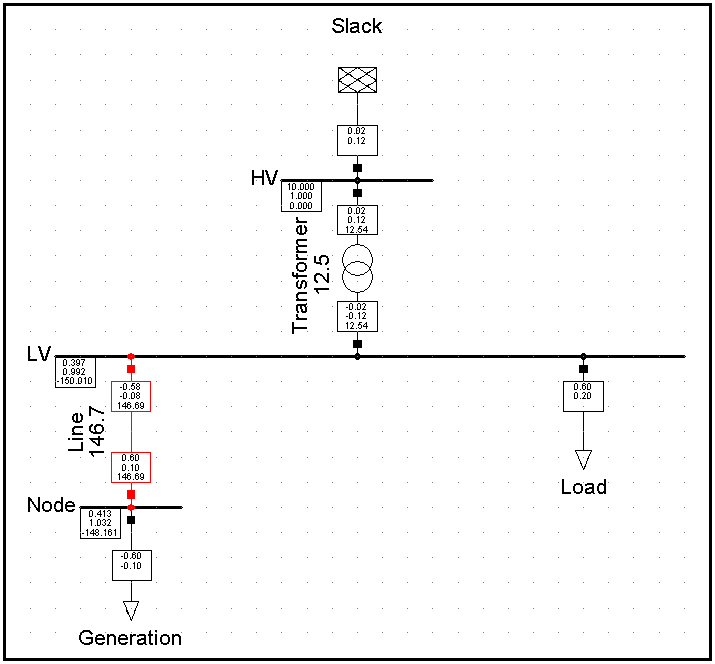
\includegraphics[width=0.8\textwidth]{test_model}}
\caption{Common network model for testing FMUs.}
\label{fig:test_model}
\end{figure}


\section{Exporting a model using external time series and triggers}
\label{sec:examples:triggers}

An example for exporting a model using external time series and triggers can be found in subfolder \texttt{test\symbol{92}triggers} of the installation folder.
It contains the following files:
\begin{itemize}
  \item \texttt{TestTriggers.pfd}: the \pf network model
  \item \texttt{TestTriggers-inputs.txt}: text file containing the lists of input variable names
  \item \texttt{TestTriggers-outputs.txt}: text file containing the lists of output variable names
  \item \texttt{TestTriggers-characteristics.csv}: text file containing a time series
\end{itemize}
In the network model, the time series is associated with the active power (parameter \texttt{plini}) of the general load named \texttt{Generation}. The time series is provided in a simple text file, using semi-colons as column separators (compare to definition of \emph{File Settings} in Figure~\ref{fig:characteristics_from_file}):
\begin{Verbatim}[frame=single,commandchars=\\\{\}]

  \textcolor{black}{1;-0.5}
  \textcolor{black}{2;-0.4}
  \textcolor{black}{3;-0.3}
  \textcolor{black}{4;-0.2}
  \textcolor{black}{5;-0.1}

\end{Verbatim}


To export the network model as FMU, issue the following command in the command prompt window (directly from the directory containing the files):
\begin{verbatim}
python.exe ..\..\powerfactory_fmu_create.py -m PFTestTriggers \
  -i TestTriggers-inputs.txt -o TestTriggers-outputs.txt \
  -p TestTriggers.pfd -t Trigger:60 TestTriggers-characteristics.csv \
  ElmLod.Load.plini=0.6
\end{verbatim}
Some comments:
\begin{itemize}
  \item This command defines \texttt{PFTestTriggers} as FMI model identifier.
  Hence, the resulting FMU is called \texttt{PFTestTriggers.fmu}.
  \item The command specifies one trigger called \texttt{Trigger}, with a scale of 60.
  This means that at master simulation time $T$ (in seconds), the associated characteristic in \pf will produce the time series value associated to $T/60$.
  For instance, at simulation time $T=180\,$s, the characteristic will produce the value $-0.3$ (compare with definition of time series above).
  \item The file containing the time series is explicitly declared as additional input file.
  In the \pf model, this file should be referred to directly by name, without a leading path (compare to Figure~\ref{fig:characteristics_from_file}).
  \item The active power (parameter name \texttt{plini} of the general load called \texttt{Load} is initialized with the value $0.6$.
\end{itemize}

\newpage

\section{Exporting a model using a \dplscript}
\label{sec:examples:dplscript}

An example for exporting a model using a \dplscript can be found in subfolder directory \texttt{test\symbol{92}dplscript} of the installation folder.
It contains the following files:
\begin{itemize}
  \item \texttt{TestDPLScript.pfd}: the \pf network model
  \item \texttt{TestDPLScript-inputs.txt}: text file containing the lists of input variable names
  \item \texttt{TestDPLScript-outputs.txt}: text file containing the lists of output variable names
\end{itemize}
In the network model, a 1-dimensional characteristic is associated with the active power (parameter \texttt{plini}) of the general load named \texttt{Generation}.
Also, the \pf model contains a \dplscript that takes the second of the year as input to set the simulation time (compare with the \dplscript shown in Section~\ref{sec:export:create_model_dplscript}).


To export the network model as FMU, issue the following command in the command prompt window (directly from the directory  containing the files):
\begin{verbatim}
python.exe ..\..\powerfactory_fmu_create.py -m PFTestDPLScript \
  -i TestDPLScript-inputs.txt -o TestDPLScript-outputs.txt \
  -p TestDPLScript.pfd -s SetTime:1:0 ElmLod.Load.plini=0.6
\end{verbatim}
Some comments:
\begin{itemize}
  \item This command defines \texttt{PFTestDPLScript} as FMI model identifier.
  Hence, the resulting FMU is called \texttt{PFTestDPLScript.fmu}.
  \item The command specifies the name of the \dplscript as \texttt{SetTime}, with a scale of 1 and an offset of 0.
  This means that at master simulation time $T$ (in seconds), the associated \dplscript will be called with an input argument value of $T/1 + 0$.
  Since in this case the \dplscript expects the second of the year as input argument, simulation time 0 coincides with the beginning of the year.
  \item The active power (parameter name \texttt{plini} of the general load called \texttt{Load} is initialized with the value $0.6$.
\end{itemize}

\section{Simulation results}
\label{sec:examples:results}

When properly exported and used within a co-simulation framework (without any further inputs), the following results should be observed for output variable \texttt{ElmTerm.Node.m:u} (FMI value reference 1001):

\begin{center}
  \begin{tabular}{|c|c|}
    \hline 
    simulation time & \texttt{ElmTerm.Node.m:u} \\ 
    \hline \hline 
    1 min & 1.026309 \\ \hline 
    2 min & 1.020366 \\ \hline 
    3 min & 1.014217 \\ \hline 
    4 min & 1.007850 \\ \hline 
    5 min & 1.001254 \\ \hline 
  \end{tabular} 
\end{center}
